% Parameter counts
% Made with Xematics. Positions are in px (1 px = 0.75 pt), as in the SVG export.
\documentclass[tikz, border=4pt]{standalone}
\definecolor{xm1}{HTML}{FFFFFF}
\definecolor{xm2}{HTML}{F1F2F4}
\definecolor{xm3}{HTML}{4B5563}
\definecolor{xm4}{HTML}{FBE8C4}
\definecolor{xm5}{HTML}{B97800}
\definecolor{xm6}{HTML}{B8C0CC}
\definecolor{xm7}{HTML}{D4E8F5}
\definecolor{xm8}{HTML}{0072B2}
\definecolor{xm9}{HTML}{DFE3E8}
\definecolor{xm10}{HTML}{AEB3B9}
\definecolor{xm11}{HTML}{6B7280}
\definecolor{xm12}{HTML}{1F2937}
\begin{document}
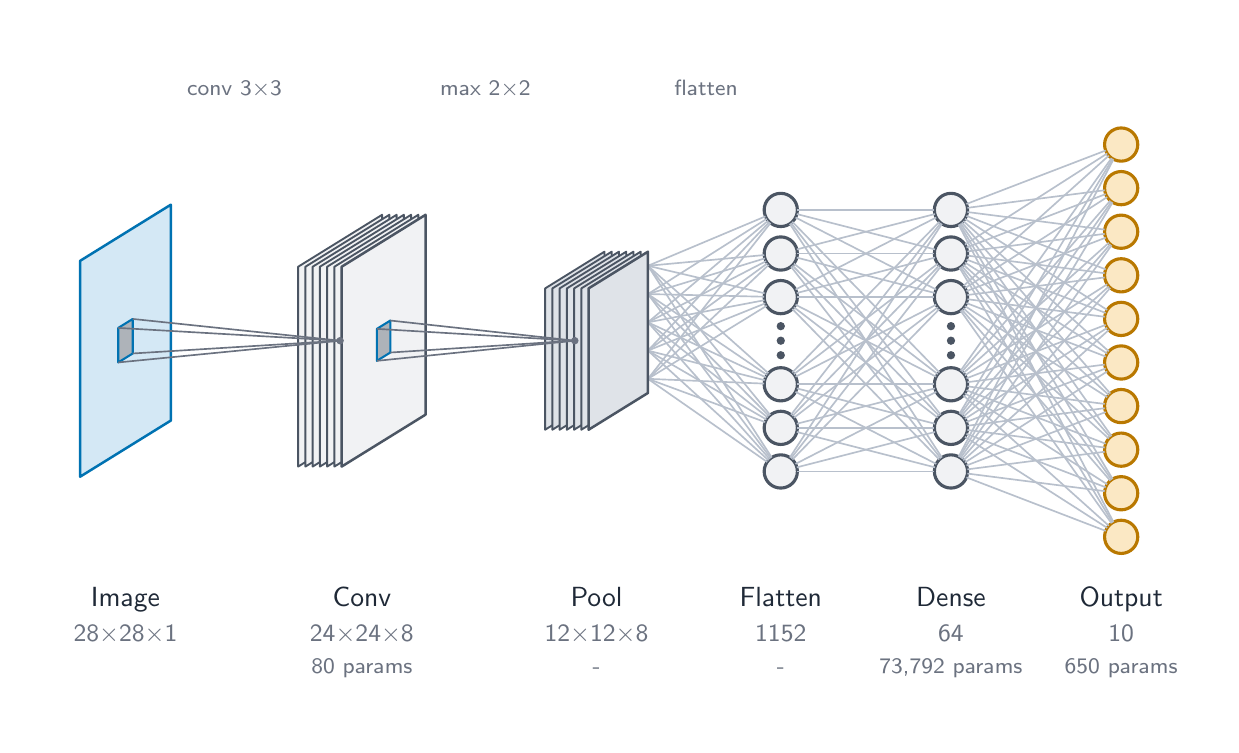
\begin{tikzpicture}[x=0.75pt, y=-0.75pt]
  \tikzset{
    xm hidden/.style={circle, minimum size=12pt, inner sep=0, outer sep=0, fill=xm2, draw=xm3, line width=1.13pt},
    xm output/.style={circle, minimum size=12pt, inner sep=0, outer sep=0, fill=xm4, draw=xm5, line width=1.13pt},
    xm edge/.style={draw=xm6, line width=0.6pt},
    xm map input/.style={fill=xm7, draw=xm8, line width=0.9pt, line join=round},
    xm map hidden back/.style={fill=xm2, draw=xm3, line width=0.68pt, line join=round},
    xm map hidden/.style={fill=xm2, draw=xm3, line width=0.9pt, line join=round},
    xm map pool back/.style={fill=xm9, draw=xm3, line width=0.68pt, line join=round},
    xm map pool/.style={fill=xm9, draw=xm3, line width=0.9pt, line join=round},
    xm dots/.style={fill=xm3},
    xm window/.style={fill=xm10, draw=xm8, line width=0.75pt, line join=round},
    xm ray/.style={draw=xm11, line width=0.6pt},
    xm ray end/.style={fill=xm11},
    xm name xm12/.style={text=xm12, inner sep=0, font=\sffamily\fontsize{9.75}{11.7}\selectfont},
    xm size xm11/.style={text=xm11, inner sep=0, font=\sffamily\fontsize{9}{10.8}\selectfont},
    xm op xm11/.style={text=xm11, inner sep=0, font=\sffamily\fontsize{8.25}{9.9}\selectfont},
    xm params xm11/.style={text=xm11, inner sep=0, font=\sffamily\fontsize{8.25}{9.9}\selectfont},
  }
  \fill[xm1] (0,0) rectangle (570.09,335.87);
  % Neurons
  \node[xm hidden] (n-3-0) at (362.84,87.81) {};
  \node[xm hidden] (n-3-1) at (362.84,108.81) {};
  \node[xm hidden] (n-3-2) at (362.84,129.81) {};
  \node[xm hidden] (n-3-1149) at (362.84,171.81) {};
  \node[xm hidden] (n-3-1150) at (362.84,192.81) {};
  \node[xm hidden] (n-3-1151) at (362.84,213.81) {};
  \node[xm hidden] (n-4-0) at (444.84,87.81) {};
  \node[xm hidden] (n-4-1) at (444.84,108.81) {};
  \node[xm hidden] (n-4-2) at (444.84,129.81) {};
  \node[xm hidden] (n-4-61) at (444.84,171.81) {};
  \node[xm hidden] (n-4-62) at (444.84,192.81) {};
  \node[xm hidden] (n-4-63) at (444.84,213.81) {};
  \node[xm output] (n-5-0) at (526.84,56.31) {};
  \node[xm output] (n-5-1) at (526.84,77.31) {};
  \node[xm output] (n-5-2) at (526.84,98.31) {};
  \node[xm output] (n-5-3) at (526.84,119.31) {};
  \node[xm output] (n-5-4) at (526.84,140.31) {};
  \node[xm output] (n-5-5) at (526.84,161.31) {};
  \node[xm output] (n-5-6) at (526.84,182.31) {};
  \node[xm output] (n-5-7) at (526.84,203.31) {};
  \node[xm output] (n-5-8) at (526.84,224.31) {};
  \node[xm output] (n-5-9) at (526.84,245.31) {};
  % Connections 2
  \draw[xm edge] (298.84,114.73) -- (n-3-0);
  \draw[xm edge] (298.84,114.73) -- (n-3-1);
  \draw[xm edge] (298.84,114.73) -- (n-3-2);
  \draw[xm edge] (298.84,114.73) -- (n-3-1149);
  \draw[xm edge] (298.84,114.73) -- (n-3-1150);
  \draw[xm edge] (298.84,114.73) -- (n-3-1151);
  \draw[xm edge] (298.84,128.34) -- (n-3-0);
  \draw[xm edge] (298.84,128.34) -- (n-3-1);
  \draw[xm edge] (298.84,128.34) -- (n-3-2);
  \draw[xm edge] (298.84,128.34) -- (n-3-1149);
  \draw[xm edge] (298.84,128.34) -- (n-3-1150);
  \draw[xm edge] (298.84,128.34) -- (n-3-1151);
  \draw[xm edge] (298.84,141.96) -- (n-3-0);
  \draw[xm edge] (298.84,141.96) -- (n-3-1);
  \draw[xm edge] (298.84,141.96) -- (n-3-2);
  \draw[xm edge] (298.84,141.96) -- (n-3-1149);
  \draw[xm edge] (298.84,141.96) -- (n-3-1150);
  \draw[xm edge] (298.84,141.96) -- (n-3-1151);
  \draw[xm edge] (298.84,155.58) -- (n-3-0);
  \draw[xm edge] (298.84,155.58) -- (n-3-1);
  \draw[xm edge] (298.84,155.58) -- (n-3-2);
  \draw[xm edge] (298.84,155.58) -- (n-3-1149);
  \draw[xm edge] (298.84,155.58) -- (n-3-1150);
  \draw[xm edge] (298.84,155.58) -- (n-3-1151);
  \draw[xm edge] (298.84,169.19) -- (n-3-0);
  \draw[xm edge] (298.84,169.19) -- (n-3-1);
  \draw[xm edge] (298.84,169.19) -- (n-3-2);
  \draw[xm edge] (298.84,169.19) -- (n-3-1149);
  \draw[xm edge] (298.84,169.19) -- (n-3-1150);
  \draw[xm edge] (298.84,169.19) -- (n-3-1151);
  % Connections 3
  \draw[xm edge] (n-3-0) -- (n-4-0);
  \draw[xm edge] (n-3-0) -- (n-4-1);
  \draw[xm edge] (n-3-0) -- (n-4-2);
  \draw[xm edge] (n-3-0) -- (n-4-61);
  \draw[xm edge] (n-3-0) -- (n-4-62);
  \draw[xm edge] (n-3-0) -- (n-4-63);
  \draw[xm edge] (n-3-1) -- (n-4-0);
  \draw[xm edge] (n-3-1) -- (n-4-1);
  \draw[xm edge] (n-3-1) -- (n-4-2);
  \draw[xm edge] (n-3-1) -- (n-4-61);
  \draw[xm edge] (n-3-1) -- (n-4-62);
  \draw[xm edge] (n-3-1) -- (n-4-63);
  \draw[xm edge] (n-3-2) -- (n-4-0);
  \draw[xm edge] (n-3-2) -- (n-4-1);
  \draw[xm edge] (n-3-2) -- (n-4-2);
  \draw[xm edge] (n-3-2) -- (n-4-61);
  \draw[xm edge] (n-3-2) -- (n-4-62);
  \draw[xm edge] (n-3-2) -- (n-4-63);
  \draw[xm edge] (n-3-1149) -- (n-4-0);
  \draw[xm edge] (n-3-1149) -- (n-4-1);
  \draw[xm edge] (n-3-1149) -- (n-4-2);
  \draw[xm edge] (n-3-1149) -- (n-4-61);
  \draw[xm edge] (n-3-1149) -- (n-4-62);
  \draw[xm edge] (n-3-1149) -- (n-4-63);
  \draw[xm edge] (n-3-1150) -- (n-4-0);
  \draw[xm edge] (n-3-1150) -- (n-4-1);
  \draw[xm edge] (n-3-1150) -- (n-4-2);
  \draw[xm edge] (n-3-1150) -- (n-4-61);
  \draw[xm edge] (n-3-1150) -- (n-4-62);
  \draw[xm edge] (n-3-1150) -- (n-4-63);
  \draw[xm edge] (n-3-1151) -- (n-4-0);
  \draw[xm edge] (n-3-1151) -- (n-4-1);
  \draw[xm edge] (n-3-1151) -- (n-4-2);
  \draw[xm edge] (n-3-1151) -- (n-4-61);
  \draw[xm edge] (n-3-1151) -- (n-4-62);
  \draw[xm edge] (n-3-1151) -- (n-4-63);
  % Connections 4
  \draw[xm edge] (n-4-0) -- (n-5-0);
  \draw[xm edge] (n-4-0) -- (n-5-1);
  \draw[xm edge] (n-4-0) -- (n-5-2);
  \draw[xm edge] (n-4-0) -- (n-5-3);
  \draw[xm edge] (n-4-0) -- (n-5-4);
  \draw[xm edge] (n-4-0) -- (n-5-5);
  \draw[xm edge] (n-4-0) -- (n-5-6);
  \draw[xm edge] (n-4-0) -- (n-5-7);
  \draw[xm edge] (n-4-0) -- (n-5-8);
  \draw[xm edge] (n-4-0) -- (n-5-9);
  \draw[xm edge] (n-4-1) -- (n-5-0);
  \draw[xm edge] (n-4-1) -- (n-5-1);
  \draw[xm edge] (n-4-1) -- (n-5-2);
  \draw[xm edge] (n-4-1) -- (n-5-3);
  \draw[xm edge] (n-4-1) -- (n-5-4);
  \draw[xm edge] (n-4-1) -- (n-5-5);
  \draw[xm edge] (n-4-1) -- (n-5-6);
  \draw[xm edge] (n-4-1) -- (n-5-7);
  \draw[xm edge] (n-4-1) -- (n-5-8);
  \draw[xm edge] (n-4-1) -- (n-5-9);
  \draw[xm edge] (n-4-2) -- (n-5-0);
  \draw[xm edge] (n-4-2) -- (n-5-1);
  \draw[xm edge] (n-4-2) -- (n-5-2);
  \draw[xm edge] (n-4-2) -- (n-5-3);
  \draw[xm edge] (n-4-2) -- (n-5-4);
  \draw[xm edge] (n-4-2) -- (n-5-5);
  \draw[xm edge] (n-4-2) -- (n-5-6);
  \draw[xm edge] (n-4-2) -- (n-5-7);
  \draw[xm edge] (n-4-2) -- (n-5-8);
  \draw[xm edge] (n-4-2) -- (n-5-9);
  \draw[xm edge] (n-4-61) -- (n-5-0);
  \draw[xm edge] (n-4-61) -- (n-5-1);
  \draw[xm edge] (n-4-61) -- (n-5-2);
  \draw[xm edge] (n-4-61) -- (n-5-3);
  \draw[xm edge] (n-4-61) -- (n-5-4);
  \draw[xm edge] (n-4-61) -- (n-5-5);
  \draw[xm edge] (n-4-61) -- (n-5-6);
  \draw[xm edge] (n-4-61) -- (n-5-7);
  \draw[xm edge] (n-4-61) -- (n-5-8);
  \draw[xm edge] (n-4-61) -- (n-5-9);
  \draw[xm edge] (n-4-62) -- (n-5-0);
  \draw[xm edge] (n-4-62) -- (n-5-1);
  \draw[xm edge] (n-4-62) -- (n-5-2);
  \draw[xm edge] (n-4-62) -- (n-5-3);
  \draw[xm edge] (n-4-62) -- (n-5-4);
  \draw[xm edge] (n-4-62) -- (n-5-5);
  \draw[xm edge] (n-4-62) -- (n-5-6);
  \draw[xm edge] (n-4-62) -- (n-5-7);
  \draw[xm edge] (n-4-62) -- (n-5-8);
  \draw[xm edge] (n-4-62) -- (n-5-9);
  \draw[xm edge] (n-4-63) -- (n-5-0);
  \draw[xm edge] (n-4-63) -- (n-5-1);
  \draw[xm edge] (n-4-63) -- (n-5-2);
  \draw[xm edge] (n-4-63) -- (n-5-3);
  \draw[xm edge] (n-4-63) -- (n-5-4);
  \draw[xm edge] (n-4-63) -- (n-5-5);
  \draw[xm edge] (n-4-63) -- (n-5-6);
  \draw[xm edge] (n-4-63) -- (n-5-7);
  \draw[xm edge] (n-4-63) -- (n-5-8);
  \draw[xm edge] (n-4-63) -- (n-5-9);
  % Layers
  \draw[xm map input] (25.28,112.33) -- (68.96,85.29) -- (68.96,189.29) -- (25.28,216.33) -- cycle;
  \draw[xm map hidden back] (130.32,115.18) -- (170.76,90.15) -- (170.76,186.44) -- (130.32,211.47) -- cycle;
  \draw[xm map hidden back] (133.81,115.18) -- (174.25,90.15) -- (174.25,186.44) -- (133.81,211.47) -- cycle;
  \draw[xm map hidden back] (137.3,115.18) -- (177.74,90.15) -- (177.74,186.44) -- (137.3,211.47) -- cycle;
  \draw[xm map hidden back] (140.79,115.18) -- (181.23,90.15) -- (181.23,186.44) -- (140.79,211.47) -- cycle;
  \draw[xm map hidden back] (144.28,115.18) -- (184.72,90.15) -- (184.72,186.44) -- (144.28,211.47) -- cycle;
  \draw[xm map hidden back] (147.77,115.18) -- (188.21,90.15) -- (188.21,186.44) -- (147.77,211.47) -- cycle;
  \draw[xm map hidden] (151.26,115.18) -- (191.7,90.15) -- (191.7,186.44) -- (151.26,211.47) -- cycle;
  \draw[xm map pool back] (249.31,125.62) -- (277.9,107.92) -- (277.9,176) -- (249.31,193.7) -- cycle;
  \draw[xm map pool back] (252.8,125.62) -- (281.39,107.92) -- (281.39,176) -- (252.8,193.7) -- cycle;
  \draw[xm map pool back] (256.29,125.62) -- (284.88,107.92) -- (284.88,176) -- (256.29,193.7) -- cycle;
  \draw[xm map pool back] (259.78,125.62) -- (288.37,107.92) -- (288.37,176) -- (259.78,193.7) -- cycle;
  \draw[xm map pool back] (263.27,125.62) -- (291.86,107.92) -- (291.86,176) -- (263.27,193.7) -- cycle;
  \draw[xm map pool back] (266.76,125.62) -- (295.35,107.92) -- (295.35,176) -- (266.76,193.7) -- cycle;
  \draw[xm map pool] (270.25,125.62) -- (298.84,107.92) -- (298.84,176) -- (270.25,193.7) -- cycle;
  \fill[xm dots] (362.84,143.81) circle[radius=2];
  \fill[xm dots] (362.84,150.81) circle[radius=2];
  \fill[xm dots] (362.84,157.81) circle[radius=2];
  \fill[xm dots] (444.84,143.81) circle[radius=2];
  \fill[xm dots] (444.84,150.81) circle[radius=2];
  \fill[xm dots] (444.84,157.81) circle[radius=2];
  \draw[xm window] (43.63,144.65) -- (50.62,140.33) -- (50.62,156.97) -- (43.63,161.29) -- cycle;
  \draw[xm ray] (43.63,144.65) -- (150.54,150.81);
  \draw[xm ray] (50.62,140.33) -- (150.54,150.81);
  \draw[xm ray] (50.62,156.97) -- (150.54,150.81);
  \draw[xm ray] (43.63,161.29) -- (150.54,150.81);
  \fill[xm ray end] (150.54,150.81) circle[radius=1.8];
  \draw[xm window] (168.25,145.11) -- (174.72,141.1) -- (174.72,156.51) -- (168.25,160.52) -- cycle;
  \draw[xm ray] (168.25,145.11) -- (263.61,150.81);
  \draw[xm ray] (174.72,141.1) -- (263.61,150.81);
  \draw[xm ray] (174.72,156.51) -- (263.61,150.81);
  \draw[xm ray] (168.25,160.52) -- (263.61,150.81);
  \fill[xm ray end] (263.61,150.81) circle[radius=1.8];
  % Labels
  \node[xm name xm12, anchor=base] at (47.12,278.9) {Image};
  \node[xm size xm11, anchor=base] at (47.12,295.66) {28\ensuremath{\times}28\ensuremath{\times}1};
  \node[xm op xm11, anchor=base] at (99.64,32.66) {conv 3\ensuremath{\times}3};
  \node[xm name xm12, anchor=base] at (161.01,278.9) {Conv};
  \node[xm size xm11, anchor=base] at (161.01,295.66) {24\ensuremath{\times}24\ensuremath{\times}8};
  \node[xm op xm11, anchor=base] at (220.5,32.66) {max 2\ensuremath{\times}2};
  \node[xm name xm12, anchor=base] at (274.08,278.9) {Pool};
  \node[xm size xm11, anchor=base] at (274.08,295.66) {12\ensuremath{\times}12\ensuremath{\times}8};
  \node[xm op xm11, anchor=base] at (326.84,32.66) {flatten};
  \node[xm name xm12, anchor=base] at (362.84,278.9) {Flatten};
  \node[xm size xm11, anchor=base] at (362.84,295.66) {1152};
  \node[xm name xm12, anchor=base] at (444.84,278.9) {Dense};
  \node[xm size xm11, anchor=base] at (444.84,295.66) {64};
  \node[xm name xm12, anchor=base] at (526.84,278.9) {Output};
  \node[xm size xm11, anchor=base] at (526.84,295.66) {10};
  \node[xm params xm11, anchor=base] at (161.01,311.21) {80 params};
  \node[xm params xm11, anchor=base] at (274.08,311.21) {-};
  \node[xm params xm11, anchor=base] at (362.84,311.21) {-};
  \node[xm params xm11, anchor=base] at (444.84,311.21) {73,792 params};
  \node[xm params xm11, anchor=base] at (526.84,311.21) {650 params};
\end{tikzpicture}
\end{document}
